\chapter{Konzeption}
\label{chapter:Konzeption}

\section{Fachliche Konzeption der Anwendung} 
\label{section:Fachliche Konzeption der Anwendung}

\subsection{Beschreibung der Anwendung}
\label{subsection:Beschreibung der Anwendung}

\subsection{Mockup der Anwendung}
\label{subsection:Mockup der Anwendung}

\begin{figure}[htbp]
\centering
		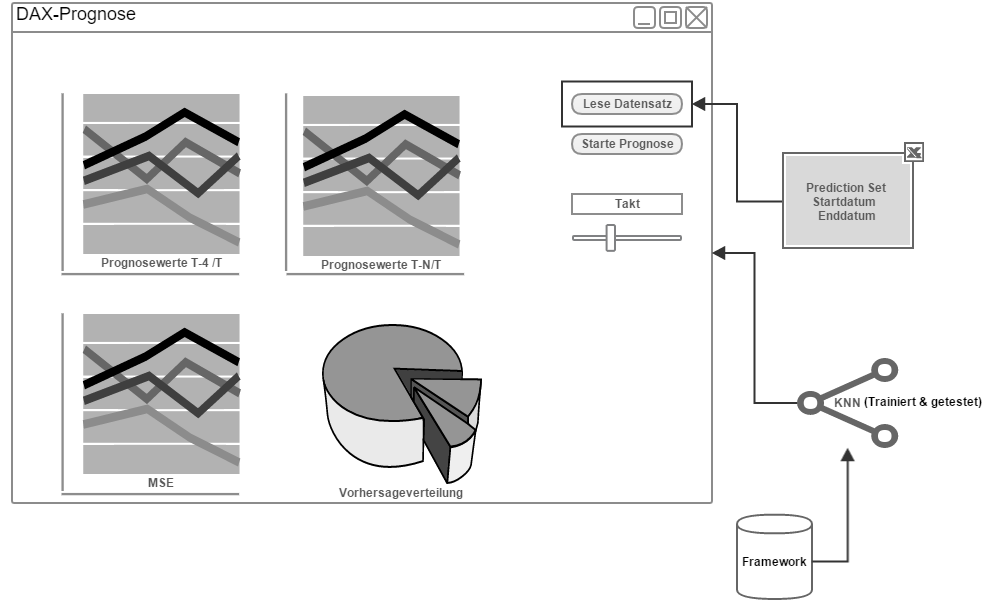
\includegraphics[width=0.95\textwidth]{mockup.PNG}
	\caption{Mockup der Anwendung}
	\label{fig:Mockup der Anwendung}
\end{figure}

\section{Konzeption des künstlichen neuronalen Netzes}
\label{section:Konzeption des künstlichen neuronalen Netzes}

in den folgenden drei Abschnitten wird auf die Konzeption des \ac{knn} eingegangen.
\subsection{Typ des künstlichen neuronalen Netzes}
\label{subsection:Typ des künstlichen neuronalen Netzes}

Grundsätzliche lassen sich \ac{knn} in zwei Oberklassen unterteilen. Die Hetero-Assoziativen Netze sowie die Auto-Assoziativen Netze. Hetero-Assoziative Netze bilden einen Vektor $A$ der Länge $n$ auf einem Vektor $B$ einer meist kürzeren Länge m $\{m \in \mathbb{N} | m \le n\}$ ab. Auto-Assoziative Netze wiederum bilden einen Eingabevektor der Länge n auf einem Ausgabevektor der gleichen Länge ab.

Innerhalb dieser zwei Klassen lassen sich \ac{knn} wiederum in mehre Modelle aufteilen. folgende Tabelle liefert eine Übersicht der bekanntesten Modelle von \ac{knn} unterteilt in Klassen:

\begin{center}
\begin{tabular}{|c|c|}
\hline 
 Hetero- assoziative Netzmodelle & Auto-assoziative Netzmodelle \\ 
\hline 
(M)Adaline & Hopfield-Netze \\ 
\hline  
Perzeptron &  Boltzmann Maschinen \\ 
\hline 
Multilayerperzeptron & - \\ 
\hline 
\end{tabular} 
\end{center}

Da es sich bei dem \ac{dax}-Kurs um einen skalaren Wert handelt, der auf Grund mehrer vorhergehender \ac{dax}-Kurse prognostiziert wird, wir ein Netzmodell aus der Klasse der Hetero-Assoziativen Netze benötigt. Für das Vorhaben ist demnach nur die linke Spalte relevant. Ein weiteres wichtiges Kriterium des benötigten Netzwerkmodells ist die Fähigkeit, mit nicht separierbaren Funktionen zu arbeiten. 

Seien $X_{0}$ and $X_{1}$ zwei Datenmengen im $n$-dimensionalen euklidischen Raum. Dann sind die Mengen $X_{0}$ and $X_{1}$ genau dann als "`linear separierbar"', wenn es  $n+1$ Werte $w_{1}, w_{2},..,w_{n}, k$, gibt, sodass jeder Punkt  $x \in X_{0}$ die Bedingung $\sum^{n}_{i=1} w_{i}x_{i} > k$ erfüllt und jeder Punkt $x \in X_{1}$ die Bedingung $\sum^{n}_{i=1} w_{i}x_{i} < k$ erfüllt.

\subsection{Grundlegende Topologie des künstlichen neuronalen Netzes}
\label{subsection:Grundlegende Topologie des künstlichen neuronalen Netzes}

\begin{figure}[H]
\centering
		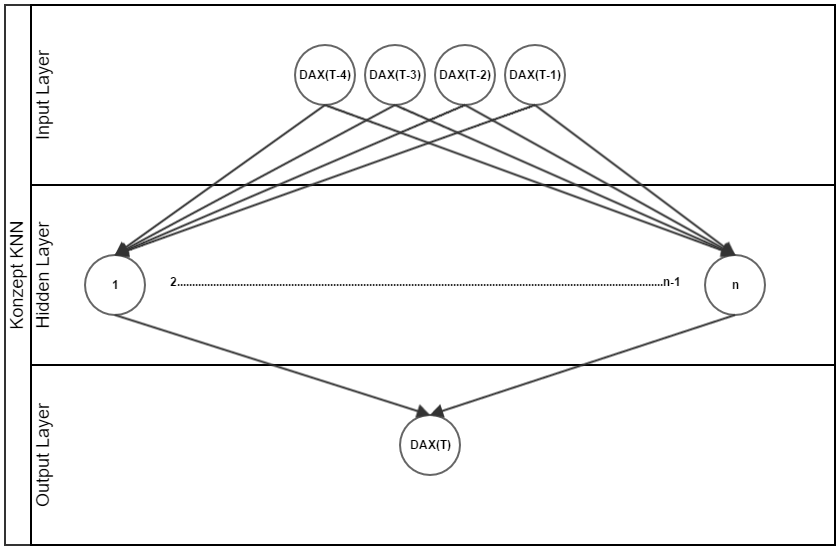
\includegraphics[width=0.95\textwidth]{KonzeptKNN.PNG}
	\caption{Grundlegendes Konzept des KNN}
	\label{fig:Grundlegendes Konzept des KNN}
\end{figure}

\subsection{Lernverfahren des künstlichen neuronalen Netzes} 
\label{subsection:Lernverfahren des künstlichen neuronalen Netzes} 

\section{Beschreibung von Frameworks} %Benedikt
\label{section:Beschreibung von Frameworks} %Benedikt

\subsection{SNNS} %Benedikt
\label{subsection:SNNS} %Benedikt

\subsection{JavaNNS}  %Benedikt
\subsection{JavaNNS}  %Benedikt

\subsection{Neuroph} %Benedikt
\label{subsection:Neuroph} %Benedikt

\section{Wahl des geeignetsten Frameworks} %Benedikt
\label{section:Wahl des geeignetsten Frameworks} %Benedikt

